\documentclass[]{article}
% bib use
\usepackage{cite}
% tabular eqn
\usepackage{amsmath, array}
% code listing
\usepackage{listings}
% images
\usepackage{graphicx} 
% lock images
\usepackage{float}


%opening
\title{Principles of statistical inference project - Part 1}
\author{Carmel Gafa'}

\begin{document}

\maketitle


\section{Question 1}

The \textbf{Exponential Distribution} is a continuous probability distribution that represents the time intervals between consecutive events in a Poisson process, where events happen independently and at a constant average rate. It is defined by a single parameter, $\lambda$, referred to as the rate parameter.


\subsection{Give reference to a publication in which the exponential distribution has been used in practise.  
	Explain the context in which this distribution has been used in this publication.}

Mahmud et al. presented a study where they analyzed and estimated response times to questions on Twitter\cite{mahmud2013will}. The authors developed predictive models to estimate response wait times, exploring three different approaches:

\begin{itemize}
	\item Personalized wait time models: These models estimate the wait time for a specific user based on their individual history of response wait times. They assume each response event for a user occurs continuously and independently at a constant average rate, modelled by an exponential distribution. Each user's rate parameter $\lambda$ is estimated as the inverse of their average past response wait times.
	
	These models demonstrated a promising ability to estimate response times on Twitter. They generally outperformed generalized models and showed reasonable accuracy, especially for an hour or more time limits. The choice of cut-off probability (a threshold used to determine whether a user is considered sufficiently likely to respond to a question on Twitter within a given period) significantly influenced the precision and recall of the predictions.
	
	\item Generalized wait time models: Instead of individual models, a single model is built using the previous responses of all users in the dataset, again using the exponential distribution. The rate parameter $\lambda$ is estimated from the responses of all users. This model underperformed compared to the personalized models in estimating response times on Twitter.
	
	
	\item Time-sensitive wait time models: These models incorporate sensitivity to the time of day or day of the week when questions are sent for both generalized and personalized models by calculating the rate parameter based on responses to questions sent during a specific day or hour. Personalized time-sensitive models only considered users with at least five responses during the modelled time interval. Incorporating time sensitivity had a modest positive impact on the generalized models but did not consistently improve the performance of the personalized models.
\end{itemize}


\subsection{State the mean and the variance of $X$.}

As $X$ follows an exponential distribution with scale parameter, $X \sim Exp(X)$, the expected value or mean is:
\begin{equation}
	E[X] = \frac{1}{\lambda}
\end{equation}
and the variance is:
\begin{equation}
	Var(X) = \frac{1}{\lambda^2}
\end{equation}


\subsection{ Derive the moment estimator of $\lambda$.}

The p.d.f. for an exponential distribution is:

\begin{equation}
	f(x)=\lambda e^{- \lambda x} \space,x \leq 0, \space \lambda > 0
\end{equation}


\noindent The first moment, or expected value:

\begin{flalign*}
E[X] &= \int_{0}^{\infty} x\space f(x) dx \\
		&= \int_{0}^{\infty} x \lambda e^{- \lambda x} dx \\
		&= \lambda \int_{0}^{\infty} x e^{- \lambda x}
\end{flalign*}

\noindent Integrating by parts, we let:

\begin{tabular}{ll}
$u = x$ 									& $du = (1) dx$ \\
$v = -\frac{e^{- \lambda x}}{\lambda}$	& $dv =  e^{- \lambda x} dx$
\end{tabular}

\bigskip
\noindent As $\int udv = uv -\int v du$:

\begin{flalign*}
E[X]	&= \lambda\left( \left[ - \frac{ x e^{- \lambda x}}{\lambda} \right]_0^\infty - \int_{0}^{\infty} -\frac{e^{- \lambda x}}{\lambda} (1) dx \right)\\
		&=   \left[ - x e^{- \lambda x}\right]_0^\infty + \int_{0}^{\infty} -e^{- \lambda x}dx
\end{flalign*}


\noindent Let us consider $\left[  x e^{- \lambda x}\right]_0^\infty$:
\begin{itemize}
	\item $- x e^{- \lambda x} = 0$, when $x=0$
	\item $\displaystyle \lim_{x \to \infty}  x e^{- \lambda x} = 0$, as exponential decay dominates polynomial growth
\end{itemize}

\noindent So the first term is removed;

\begin{flalign*}
	E[X] &=\int_{0}^{\infty} -e^{- \lambda x}dx\\
		&= \left[  -\frac{1}{\lambda} -e^{- \lambda x} \right]_0^\infty\\
		&= 0 - \left( - \frac{1}{\lambda}\right)\\
		&= \frac{1}{\lambda}
\end{flalign*}

\noindent As in the method of moments the sample mean is equal to theoretical expectation;
$$
E[X] = \frac{1}{\lambda}=\overline{X}
$$

\noindent and solving for $\lambda$

\begin{equation}
	\hat{\lambda} = \frac{1}{\overline{X}}
\end{equation}

\subsection{Use the second moment to obtain another estimator of $\lambda$}

For an exponential distribution with rate parameter $\lambda$, the second moment,

\begin{flalign*}
	E[X^2] &= \int_{0}^{\infty} x^2 \space f(x) dx \\
	&= \int_{0}^{\infty} x^2 \lambda e^{- \lambda x} dx \\
	&= \lambda \int_{0}^{\infty} x^2 e^{- \lambda x}
\end{flalign*}

\noindent We let:

\begin{tabular}{ll}
	$u = x^2$ 									& $du = 2x dx$ \\
	$v = -\frac{e^{- \lambda x}}{\lambda}$	& $dv =  e^{- \lambda x} dx$
\end{tabular}

\begin{flalign*}
	E[X^2]	&= \lambda\left( \left[ - \frac{ x^2 e^{- \lambda x}}{\lambda} \right]_0^\infty - \int_{0}^{\infty} -\frac{e^{- \lambda x}}{\lambda} 2x dx \right)\\
	&=   \left[ - x^2 e^{- \lambda x}\right]_0^\infty + \int_{0}^{\infty} 2xe^{- \lambda x}dx
\end{flalign*}

\noindent Let us consider $\left[  x^2 e^{- \lambda x}\right]_0^\infty$:
\begin{itemize}
	\item $- x^2 e^{- \lambda x} = 0$, when $x=0$
	\item $\displaystyle \lim_{x \to \infty}  x^2 e^{- \lambda x} = 0$, as exponential decay dominates polynomial growth
\end{itemize}

Then

$$E[X^2] =  \int_{0}^{\infty} 2xe^{- \lambda x}dx$$

\noindent We let:

\begin{tabular}{ll}
	$u = x$ 									& $du = dx$ \\
	$v = -\frac{e^{- \lambda x}}{\lambda}$	& $dv =  e^{- \lambda x} dx$
\end{tabular}

$$E[X^2] = 2\left(  \left[  -\frac{xe^{- \lambda x}}{\lambda} \right] - \int_{0}^{\infty} e^{- \lambda x}dx \right)$$

\noindent We have seen previously that the first term will equate to zero.

\begin{flalign*}
	E[X^2]	&= 2  \int_{0}^{\infty} \frac{e^{- \lambda x}}{\lambda} dx \\
			&= \left[ - \frac{2 e^{- \lambda x}}{\lambda^2} \right]_0^\infty \\
			&= 0-\left(-\frac{2}{\lambda^2}\right) \\
			& = \frac{2}{\lambda^2}
\end{flalign*}


\noindent The variance of the exponential distribution is given by:

\begin{flalign*}
	Var(X)	&= E[X^2] - E[X]^2\\
			&= \frac{2}{\lambda^2} - \left(\frac{1}{\lambda}\right)^2\\
			&= \frac{1}{\lambda^2}
\end{flalign*}

\noindent We can estimate the sample variance

$$\hat{\sigma}^2 = \frac{1}{\hat{\lambda}^2}$$

\noindent and solving for $\lambda$

\begin{equation}
	\hat{\lambda} = \frac{1}{\sqrt{\hat{\sigma}^2}}
\end{equation}


\subsection{Comment on the unbiasedness and consistency of the moment estimator for $\lambda$ derived in Q1iii.
	State any assumption/s that need to be made to check for unbiasedness and consistency.}

\subsection{Use R software to generate 1000 data points from an exponential distributed random variable using
	any admissible parameter value for $\lambda$}

The R script generates 1000 points from an exponentially distributed random variable with a rate parameter $\lambda$ of 1.5. It then plots a histogram of these points and overlays the theoretical density function of the exponential distribution. The result is shown in Figure \ref{fig:img-1-6-1}.


\begin{lstlisting}
library(ggplot2)
library(glue)

set.seed(50)
lambda <- 1.5
x <- rexp(n = 1000, rate = lambda)

data <- data.frame(x = x)

p <- ggplot(data,
		aes(x = x)) +
	geom_histogram(
		aes(y = after_stat(density)),
		bins = 50, fill = "blue",
		color = "black",
		alpha = 0.6) +
	stat_function(
		fun = function(x) lambda * exp(-lambda * x),
		color = "red",
		size = 1) +
	labs(title = glue("Histogram of exponentially distributed 
	random variable with lambda = {lambda}"),
		x = "x", y = "Density") +
	theme_minimal() +
	theme(plot.title = element_text(hjust = 0.5))
\end{lstlisting}


\begin{figure}[H]
	\centering
	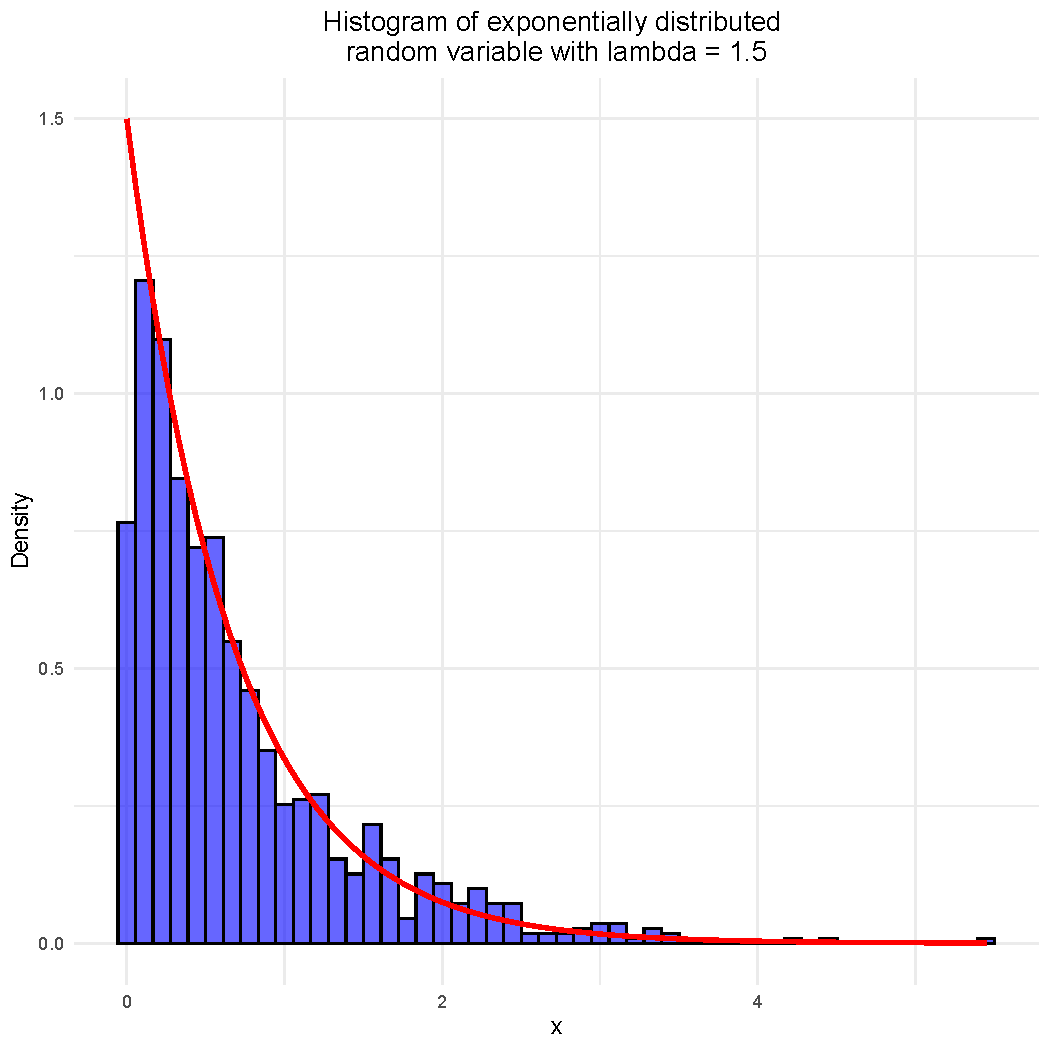
\includegraphics[width=0.7\linewidth]{img/img-1-5-1.jpeg}
	\caption{Exponential distributed random variable; histogram of 1000 generated points and theoretical distribution}
	\label{fig:img-1-6-1}
\end{figure}

\subsubsection{Write down the log-likelihood function for this exponentially distributed random variable.}

For sample $\mathbf{x} = ( x_1, \dots, x_n )^T$ obtained on an exponential distributed random variable $X$, with parameter vector $\mathbf{\theta}=(\lambda)$, the likelihood


\begin{flalign*}
	L(\mathbf{x}, \mathbf{\theta})	&= \prod_{i=1}^{n} f(x_i, \mathbf{\theta}) \\
		&=  \prod_{i=1}^{n} \lambda e^{-\lambda x_i} \\
		&= \lambda^n e^{\sum_{i=1}^n \lambda x_i}
\end{flalign*}

\noindent The log-likelihood is then

$$	
l(\mathbf{x}, \mathbf{\theta}) = n \space log(\lambda) - \lambda \sum_{i=0}^{n} x_i	
$$

\noindent Taking the derivative with respect to $\lambda$,

$$
\frac{\partial l(\mathbf{x}, \mathbf{\theta}) }{\partial\lambda} =
\frac{n}{\lambda} - \sum_{i=0}^{n} x_i	
$$

\noindent for maximum $\frac{\partial l(\mathbf{x}, \mathbf{\theta}) }{\partial\lambda}$

\begin{flalign*}
	L\frac{\partial l(\mathbf{x}, \mathbf{\theta}) }{\partial\lambda}	&= 0 \\ 
	\frac{n}{\lambda} - \sum_{i=0}^{n} x_i	 &= 0 \\
	\frac{n}{\lambda}  &= \sum_{i=0}^{n} x_i	
\end{flalign*}

\noindent So that

\begin{equation}
	\hat{\lambda} = \frac{n}{\sum_{i=0}^{n} x_i	} = \frac{1}{\overline{x}}
\end{equation}


\subsubsection{Evaluate the log-likelihood function for the generated data as a function of $\lambda$, and plot the resulting log-likelihood function against different values of $\lambda$. Present the plot together with the answers.}


The follwoing listing calculates and plots the log-likelihood values for an exponential distribution with varying $\lambda$ values. The resulting plot can be examined in Figure \ref{fig:img-1-6-2}


\begin{lstlisting}
	lambda_values <- seq(0.1, 5, by = 0.01)
	log_likelihood_values <- sapply(lambda_values,
	function(lambda) LL_exponential(lambda, x))
	
	df <- data.frame(lambda_values, log_likelihood_values)
	
	p <- ggplot(df, 
		aes(x = lambda_values, 
		y = log_likelihood_values)) +
	geom_point(
		color = "blue",
		alpha = 0.6) +
		labs(
		title = "Log-Likelihood with varying
		 lambda values",
		x = "Lambda",
		y = "Log-Likelihood") +
	theme_bw()
	
	quartz()
	print(p)
\end{lstlisting}

\begin{figure}[H]
	\centering
	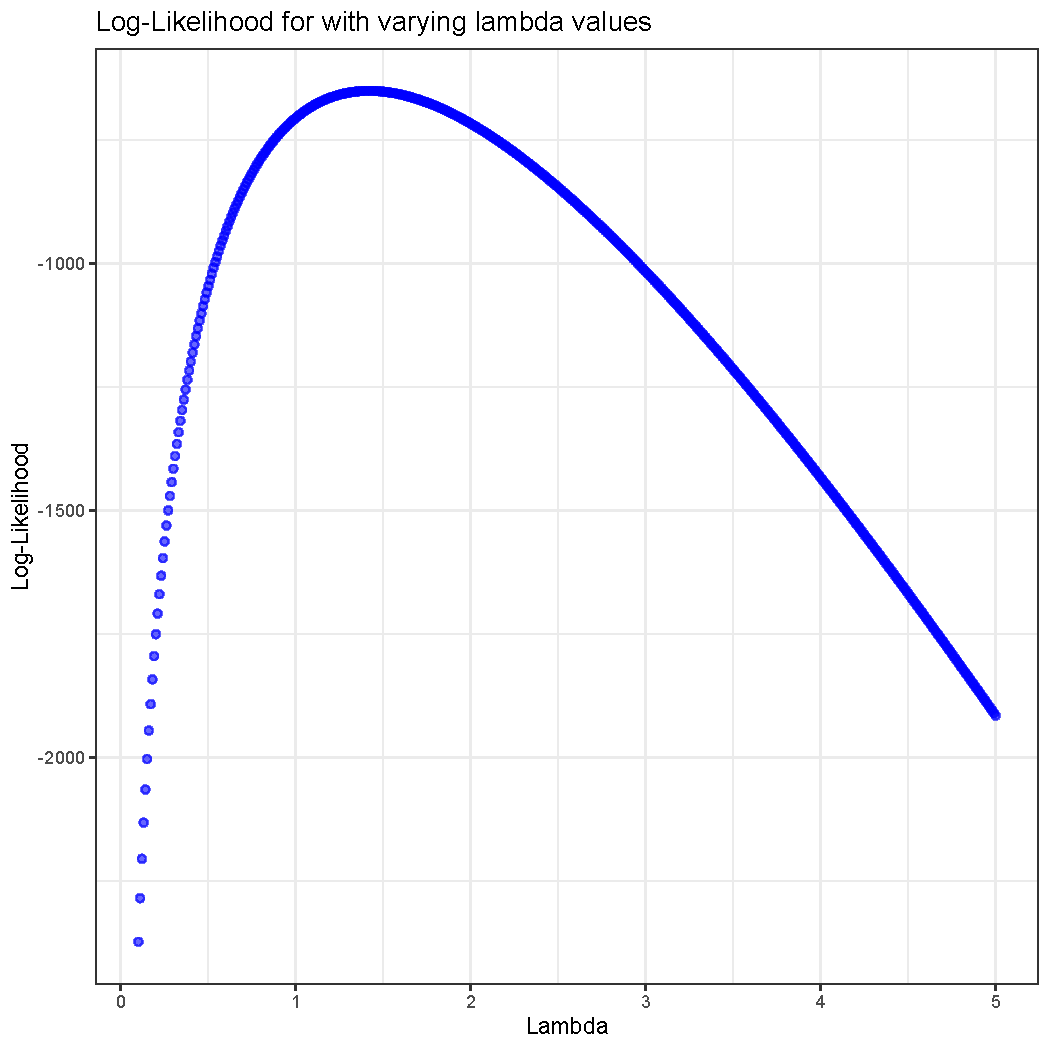
\includegraphics[width=0.7\linewidth]{img/img-1-6-2.jpeg}
	\caption{Log-likelihood plot for an exponential distribution with varying $\lambda$}
	\label{fig:img-1-6-2}
\end{figure}


\subsubsection{Using the plot or otherwise, which estimate for $\lambda$ is the MLE? Give a reason for your answer.}

As we have seen in the previous question, the maximum likelihood estimation is the value for which the derivative of the log-likelihood with respect to lambda is zero, that is the peak of the curve shown in Figure \ref*{fig:img-1-6-2}. This can be easily calculated using the code below. The value obtained for $\hat{\lambda}$ was \textbf{1.43}.

\begin{lstlisting}
max_ll <- max(log_likelihood_values)
max_lambda <- lambda_values[log_likelihood_values == max_ll]
print(glue("Lambda value for maximum log-likelihood is {max_lambda}"))
\end{lstlisting}




\bibliography{references}
\bibliographystyle{plain}



\end{document}